
\documentclass[a4paper,11pt]{article}
\usepackage[a4paper, margin=8em]{geometry}

% usa i pacchetti per la scrittura in italiano
\usepackage[french,italian]{babel}
\usepackage[T1]{fontenc}
\usepackage[utf8]{inputenc}
\frenchspacing 

% usa i pacchetti per la formattazione matematica
\usepackage{amsmath, amssymb, amsthm, amsfonts}

% usa altri pacchetti
\usepackage{gensymb}
\usepackage{hyperref}
\usepackage{standalone}

% imposta il titolo
\title{Appunti Elettronica Digitale}
\author{Luca Seggiani}
\date{2026}

% imposta lo stile
% usa helvetica
\usepackage[scaled]{helvet}
% usa palatino
\usepackage{palatino}
% usa un font monospazio guardabile
\usepackage{lmodern}

\renewcommand{\rmdefault}{ppl}
\renewcommand{\sfdefault}{phv}
\renewcommand{\ttdefault}{lmtt}

% disponi il titolo
\makeatletter
\renewcommand{\maketitle} {
	\begin{center} 
		\begin{minipage}[t]{.8\textwidth}
			\textsf{\huge\bfseries \@title} 
		\end{minipage}%
		\begin{minipage}[t]{.2\textwidth}
			\raggedleft \vspace{-1.65em}
			\textsf{\small \@author} \vfill
			\textsf{\small \@date}
		\end{minipage}
		\par
	\end{center}

	\thispagestyle{empty}
	\pagestyle{fancy}
}
\makeatother

% disponi teoremi
\usepackage{tcolorbox}
\newtcolorbox[auto counter, number within=section]{theorem}[2][]{%
	colback=blue!10, 
	colframe=blue!40!black, 
	sharp corners=northwest,
	fonttitle=\sffamily\bfseries, 
	title=~\thetcbcounter: #2, 
	#1
}

% disponi definizioni
\newtcolorbox[auto counter, number within=section]{definition}[2][]{%
	colback=red!10,
	colframe=red!40!black,
	sharp corners=northwest,
	fonttitle=\sffamily\bfseries,
	title=~\thetcbcounter: #2,
	#1
}

% U.D.M
\newcommand{\amp}{\ensuremath{\mathrm{A}}}
\newcommand{\volt}{\ensuremath{\mathrm{V}}}
\newcommand{\meter}{\ensuremath{\mathrm{m}}}
\newcommand{\second}{\ensuremath{\mathrm{s}}}
\newcommand{\farad}{\ensuremath{\mathrm{F}}}
\newcommand{\henry}{\ensuremath{\mathrm{H}}}
\newcommand{\siemens}{\ensuremath{\mathrm{S}}}

% circuiti
\usepackage{circuitikz}
\usetikzlibrary{babel}

% disegni
\usepackage{pgfplots}
\pgfplotsset{width=10cm,compat=1.9}

% disponi codice
\usepackage{listings}
\usepackage[table]{xcolor}

\definecolor{codegreen}{rgb}{0,0.6,0}
\definecolor{codegray}{rgb}{0.5,0.5,0.5}
\definecolor{codepurple}{rgb}{0.58,0,0.82}
\definecolor{backcolour}{rgb}{0.95,0.95,0.92}

\lstdefinestyle{codestyle}{
		backgroundcolor=\color{black!5}, 
		commentstyle=\color{codegreen},
		keywordstyle=\bfseries\color{magenta},
		numberstyle=\sffamily\tiny\color{black!60},
		stringstyle=\color{green!50!black},
		basicstyle=\ttfamily\footnotesize,
		breakatwhitespace=false,         
		breaklines=true,                 
		captionpos=b,                    
		keepspaces=true,                 
		numbers=left,                    
		numbersep=5pt,                  
		showspaces=false,                
		showstringspaces=false,
		showtabs=false,                  
		tabsize=2
}

\lstdefinestyle{shellstyle}{
		backgroundcolor=\color{black!5}, 
		basicstyle=\ttfamily\footnotesize\color{black}, 
		commentstyle=\color{black}, 
		keywordstyle=\color{black},
		numberstyle=\color{black!5},
		stringstyle=\color{black}, 
		showspaces=false,
		showstringspaces=false, 
		showtabs=false, 
		tabsize=2, 
		numbers=none, 
		breaklines=true
}

\lstdefinelanguage{javascript}{
	keywords={typeof, new, true, false, catch, function, return, null, catch, switch, var, if, in, while, do, else, case, break},
	keywordstyle=\color{blue}\bfseries,
	ndkeywords={class, export, boolean, throw, implements, import, this},
	ndkeywordstyle=\color{darkgray}\bfseries,
	identifierstyle=\color{black},
	sensitive=false,
	comment=[l]{//},
	morecomment=[s]{/*}{*/},
	commentstyle=\color{purple}\ttfamily,
	stringstyle=\color{red}\ttfamily,
	morestring=[b]',
	morestring=[b]"
}

% disponi sezioni
\usepackage{titlesec}

\titleformat{\section}
	{\sffamily\Large\bfseries} 
	{\thesection}{1em}{} 
\titleformat{\subsection}
	{\sffamily\large\bfseries}   
	{\thesubsection}{1em}{} 
\titleformat{\subsubsection}
	{\sffamily\normalsize\bfseries} 
	{\thesubsubsection}{1em}{}

% disponi alberi
\usepackage{forest}

\forestset{
	rectstyle/.style={
		for tree={rectangle,draw,font=\large\sffamily}
	},
	roundstyle/.style={
		for tree={circle,draw,font=\large}
	}
}

% disponi algoritmi
\usepackage{algorithm}
\usepackage{algorithmic}
\makeatletter
\renewcommand{\ALG@name}{Algoritmo}
\makeatother

% disponi numeri di pagina
\usepackage{fancyhdr}
\fancyhf{} 
\fancyfoot[L]{\sffamily{\thepage}}

\makeatletter
\fancyhead[L]{\raisebox{1ex}[0pt][0pt]{\sffamily{\@title \ \@date}}} 
\fancyhead[R]{\raisebox{1ex}[0pt][0pt]{\sffamily{\@author}}}
\makeatother

\begin{document}
% sezione (data)
\section{Lezione del 20-04-26}

% stili pagina
\thispagestyle{empty}
\pagestyle{fancy}

% testo
Abbiamo visto la rete di polarizzazione del MOSFET NMOS a 4 resistori, e come questa ci permetteva di stabilizzare il comportamento del componente riconducendolo alle resistenze esterne. 

Ci resta quindi da vedere il modello per i \textit{piccoli segnali}.
In tal caso prendiamo il modello generale del MOSFET in saturazione:
$$
i_D = \mu_n C_{ox} \frac{W}{L} \frac{(V_{GS} - V_T)^2}{2} (1 + \lambda V_{DS})
$$
dove abbiamo incluso il termine di \textit{modulazione di canale} (visto in 16.0.1).

\subsubsection{Conduttanza e resistenza differenziale}
Il modello ai piccoli segnali del MOSFET, come abbiamo visto in 16.1, è sempre un circuito con gate e source isolati (conta solo la tensione fra questi), e dove se consideriamo il termine di modulazione di canale abbiamo fra drain e source 2 componenti (in parallelo):
\begin{enumerate}
	\item Un generatore di corrente pilotato in tensione:
		$$
		g_m v_{gs}
		$$
		dove la $g_m$ viene detta \textit{conduttanza differenziale};
	\item Una resistenza differenziale in parallelo:
		$$
		r_d
		$$
		dove la $r_d$ viene detta appunto \textit{resistenza differenziale}.
\end{enumerate}

\newpage

Il circuito si presenta quindi come segue:
\begin{center}
\begin{tikzpicture}[transform shape]
	% Paths, nodes and wires:
	\draw (4, 6) to[open, o-o] (6, 6);
	\draw (4, 6) |- (2, 6);
	\draw (6, 6) -- (10, 6);
	\draw (2, 4) -- (10, 4);
	\node[shape=rectangle, minimum width=0.465cm, minimum height=0.465cm] at (4, 6.25){} node[anchor=center, align=center, text width=0.077cm, inner sep=6pt] at (4, 6.25){G};
	\node[shape=rectangle, minimum width=0.465cm, minimum height=0.465cm] at (6, 6.25){} node[anchor=center, align=center, text width=0.077cm, inner sep=6pt] at (6, 6.25){D};
	\node[shape=rectangle, minimum width=0.465cm, minimum height=0.465cm] at (6, 3.75){} node[anchor=center, align=center, text width=0.077cm, inner sep=6pt] at (6, 3.75){S};
	\draw (2, 6) to[open, v=$v_{gs}$, voltage=american] (2, 4);
	\draw (10, 6) to[open, v=$v_{ds}$, voltage=american] (10, 4);
	\draw (6, 6) to[american controlled current source, l={$g_m v_{gs}$}] (6, 4);
	\draw (8, 6) to[american resistor, l={$r_d$}] (8, 4);
\end{tikzpicture}
\end{center}

Conduttanza e resistenza differenziale si calcolano come linearizzazione del modello del MOSFET, rispettivamente su $V_{GS}$ e $V_{DS}$:
$$
g_m = \frac{\partial i_D}{\partial V_{GS}} \Big|_Q, \quad
r_d = \frac{\partial V_{DS}}{\partial i_{D}} = \left( \frac{\partial i_{D}}{\partial V_{DS}} \right)^{-1}
$$
dove $Q$ è il punto di quiescenza, secondo un procedimento analogo alla linearizzazione del diodo (9.1) o del transistore bipolare (sezione 12.1).
Svogliamo i calcoli:
\begin{itemize}
\item Per $g_m$ abbiamo la derivata del modello su $V_{GS}$, per cui:
$$
g_m = \frac{\partial i_D}{\partial V_{GS}} \Big|_Q = \left(\mu_n C_{ox} \frac{W}{L}\right) \frac{1}{2} 2 (V_{GS} - V_T) (1 + \lambda V_{DS}) \approx \frac{2 I_D}{V_{GS} - V_T} = K(V_{GS} - V_T)
$$
dove notiamo l'approssimazione che trascura l'effetto di modulazione di canale.
Ricordiamo anche che i valori in maiuscolo relativi al punto di quiescenza;
\item Per $r_d$ abbiamo l'inverso della derivata del modello su $V_{DS}$, per cui:
$$
r_d = \left( \frac{\partial i_D}{\partial V_{DS}}  \Big|_Q \right)^{-1}
= \left( K \frac{(V_{GS} - V_T)^2}{2} \lambda \right)^{-1} = \frac{1 + \lambda V_{DS}}{\lambda I_D} \approx \frac{1}{\lambda I_D}
$$
dove notiamo l'approssimazione se $\lambda V_{DS} << 1$.
Solitamente, poi, notiamo che $r_d$ viene trascurata nei casi reali (in quanto è solitamente molto grande, la assumiamo $\rightarrow \infty$). Questa è un approssimazione valida per i componenti discreti, ma notiamo che non lo è per i circuiti integrati (dove diventa abbastanza bassa da dover essere considerata). 
\end{itemize}

\par\smallskip

Finora abbiamo visto il caso NMOS. Ci potremmo chiedere se il modello per il PMOS si comporta in maniera equivalente. Ad esempio, avevamo che per il punto di riposo del PMOS si aveva il senso delle correnti invertito (si considerava $I_{SD}$ anziché $I_{DS}$).

Per i piccoli segnali, invece, il generatore di corrente ha lo stesso identico segno e il modello non cambia (i cambiamenti di segno sono inclusi nelle equazioni, col fatto che la $V_{GS}$ e la $V_{DS}$ saranno negative). 

\subsubsection{Caratteristiche a source comune}
Iniziamo a vedere le configurazioni standard del MOSFET, esattamente nello stesso modo in cui le avevamo viste per il BJT.

\begin{center}
\begin{circuitikz}
	\draw
(0,0) node[ground]{} to[R=$R_2$] (0,3)
to[R=$R_1$] (0,6) node[vcc]{};

\draw (0,3) -- (2,3);

\draw (2,3) node[nmos, anchor=B] (Q1) {};

\draw (Q1.C) to[R=$R_D$] ++(0,3) node[vcc]{};
\draw (Q1.E) to[R=$R_S$] ++(0,-3) node[ground]{};

\draw[->] (1.2,3.3) -- (1.8,3.3) node[midway, above]{$I_G$};
\draw[->] (Q1.C) ++(0.3,0.5) -- ++(0,-1) node[midway, right]{$I_D$};
\draw[->] (Q1.E) ++(0.3,0) -- ++(0,-.8) node[midway, right]{$I_S$};

\node[ground] at(-4, 0) {};
\draw (-4, 0) to [ voltage source, v=$V_i$] (-4,3)
	to [resistor, l=$R_s$] (-2, 3)
	to [capacitor, l=$C_s$] (0, 3);

\node[ground] at(6, 0) {};
\draw(3, 4.5) to[ capacitor, l=$C_L$] (6, 4.5)
	to[resistor, l=$R_L$] (6, 0);

\end{circuitikz}
\end{center}

Assumiamo di aver già considerato il punto di quiescenza e passiamo direttamente alla risposta ai piccoli segnali. In tal caso le capacità di accoppiamento AC sono trascurate, e prendiamo a sinistra le resistenze di polarizzazione in parallelo al ground. Per il MOSFET prendiamo il modello ai piccoli segnali, e notiamo che tutto il lato "segnale" del circuito (fino al gate) viene effettivamente separato dal lato di destra.
Il circuito (cortesia della collega Imane) ai piccoli segnali si presenta allora come segue:
\begin{center}
	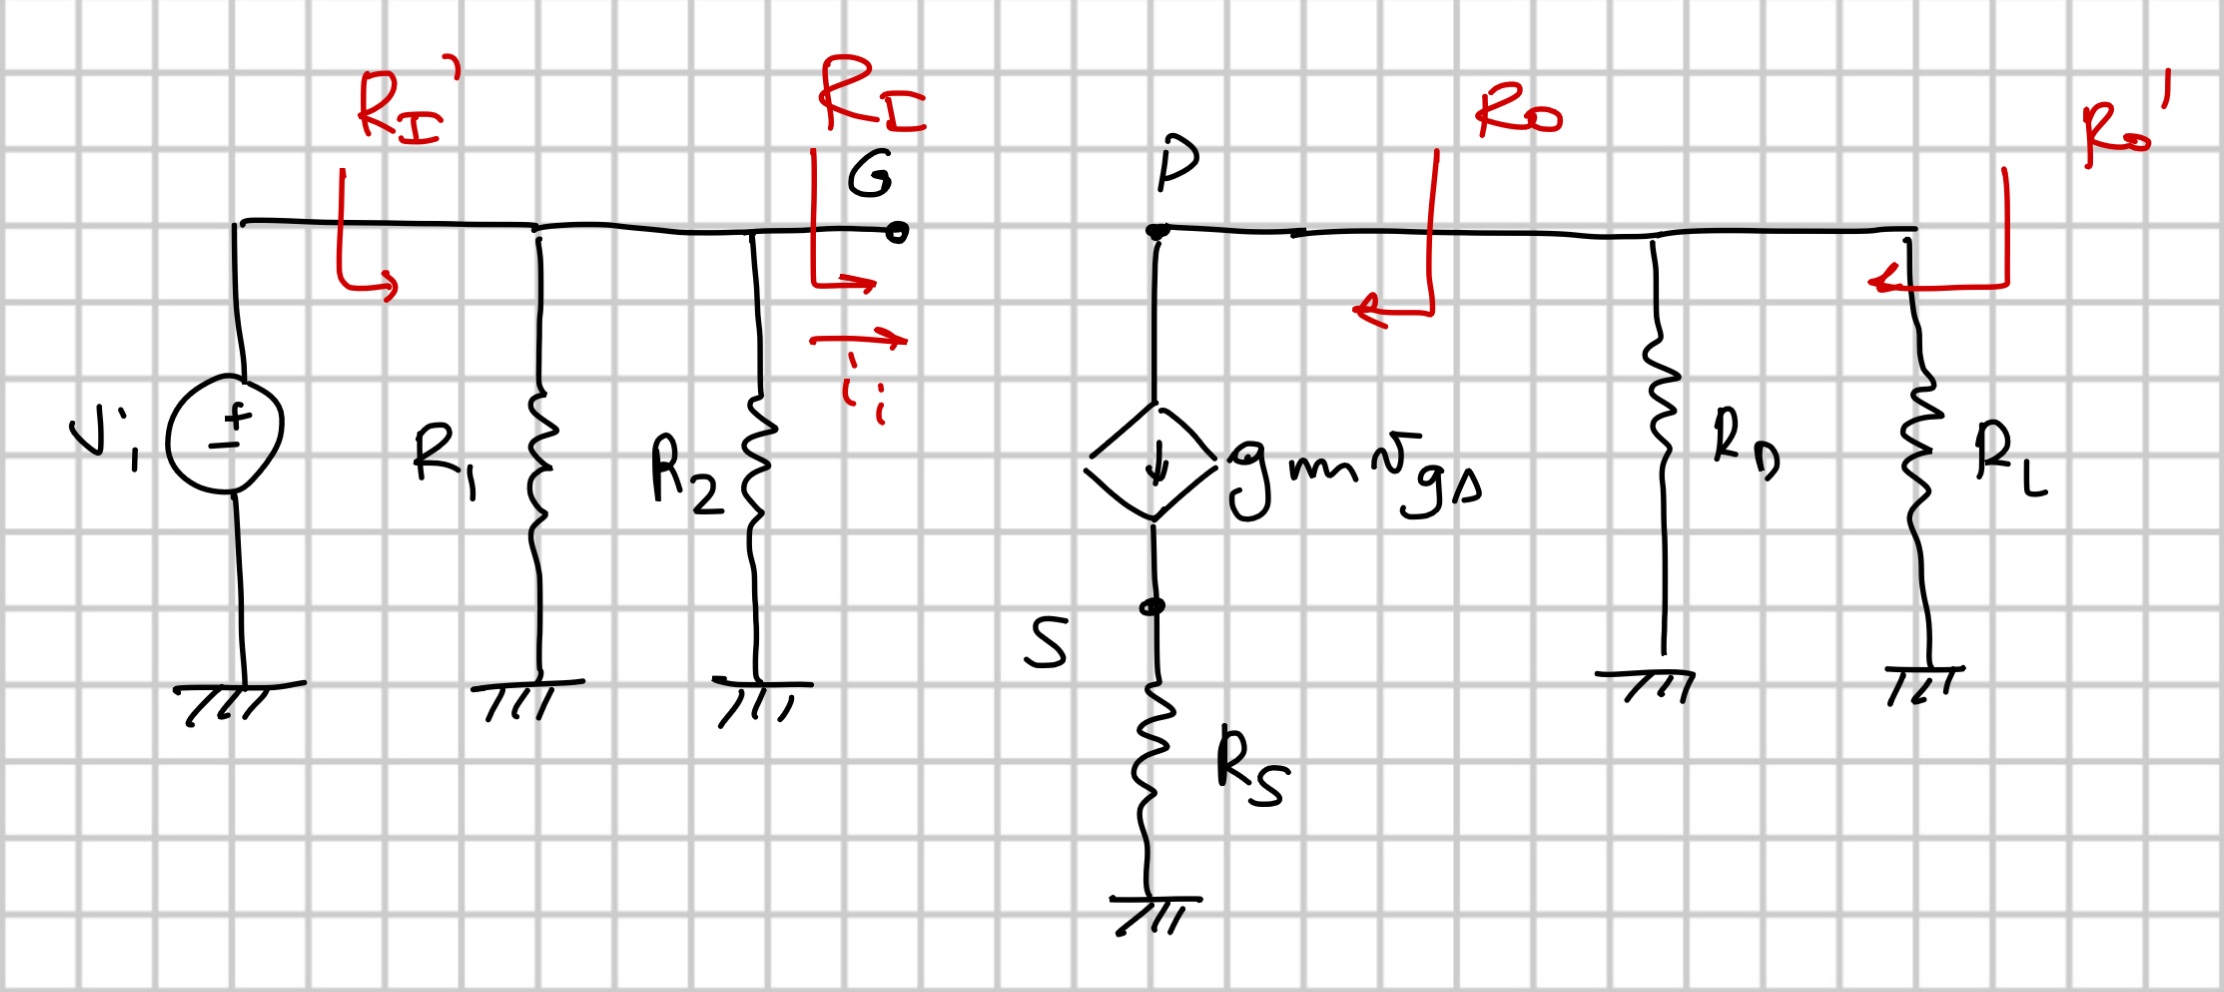
\includegraphics[scale=0.15]{../figures/mosfet_source_imane.png}
\end{center}

Calcoliamo quindi i parametri caratteristici:
\begin{itemize}
\item \textbf{\textsf{Guadagno di tensione}} $A_v$ \\
Per il guadagno di tensione consideriamo il rapporto fra la tensione in uscita e quella in ingresso. La prima sarà data esclusivamente dalla caduta sulla $R_D$, in quanto il gate è separato dal resto del circuito:
$$
v_o = - g_m v_{gs} R_D
$$
Vediamo quindi la $v_{gs}$:
$$
\begin{cases}
v_{gs} = v_g - v_s \\
v_s = g_m v_{gs} R_S
\end{cases}, \quad
v_{gs} = v_g - R_S g_m v_{gs} \implies
v_{gs} = \frac{v_g}{1 + g_m R_s}
$$

A questo punto accorgiamoci che la $v_i$ non è altro che la $v_g$ che imponiamo al gate del MOSFET, per cui:
$$
A_v = \frac{v_o}{v_i} \Big|_{R_L \rightarrow \infty} = -\frac{g_m R_D}{1 + g_m R_S}
$$

Notiamo subito che la configurazione a source comune è \textit{invertente}, in quanto si ha un guadagno di tensione negativo. Valgono le solite euristiche, cioè:
\begin{itemize}
\item Se $R_S = 0$, si ha:
$$
A_v = - g_m R_D
$$
dove $g_m$ è altamente variabile (dipende dal MOSFET);
\item Se $g_m R_S >> 1$, condizione che non è difficile da ottenere, si ha:
$$
A_v \approx -\frac{R_D}{R_S}
$$
cioè abbiamo riportato il guadagno in qualcosa che non dipende (o almeno dipende in parte minima) dalle caratteristiche del MOSFET, e che è facile da calcolare, cosa che ci rende quantomai felici.
\end{itemize}

\item \textbf{\textsf{Guadagno di corrente}} $A_i$ \\
Il guadagno di corrente andrà ad infinito per il fatto che la corrente in ingresso sarà nulla (questo perché il gate è separato dal resto MOSFET, lo vedremo meglio nel calcolo della $R_i$). Avremo quindi:
$$
A_i = \frac{i_o}{i_i} \rightarrow \infty
$$

\item \textbf{\textsf{Impedenza in uscita}} $R_o$ \\
Per l'impedenza in uscita mettiamo un generatore di prova al drain, e spengiamo il generatore di segnale.
$$
\begin{cases}
v_g = 0 \\
v_s = R_S g_m v_{gs} \\
v_{gs} = v_g - v_s = - v_s
\end{cases}, \quad
v_s = R_s g_m (- v_s) \implies v_s = 0, \quad v_{gs} = 0
$$
e quindi il generatore pilotato non è spento è la corrente è nulla. Da questo deriva impedenza infinita all'uscità, cioè:
$$
R_o \rightarrow \infty
$$
Chiaramente, un eventuale carico $R_L$ vedrà la resistenza data dal parallelo $R_D || R_L$. 

\item \textbf{\textsf{Impedenza in ingresso}} $R_i$ \\
Questa è banale in quanto il gate è separato dal resto del MOSFET, per cui da questo si vedrà impedenza infinita:
$$
R_i \rightarrow \infty
$$
Chiaramente, anche qui, il generatore $V_i$ vedrà invece il solo parallelo $R_1||R_2$.
\end{itemize}

\subsubsection{Caratteristiche a drain comune}
Vediamo anche le caratteristiche a drain comune, dove preleviamo il segnale di uscita dal source anziché dal drain.

\begin{center}
\begin{circuitikz}
	\draw
(0,0) node[ground]{} to[R=$R_2$] (0,3)
to[R=$R_1$] (0,6) node[vcc]{};

\draw (0,3) -- (2,3);

\draw (2,3) node[nmos, anchor=B] (Q1) {};

\draw (Q1.C) to[short] ++(0,3) node[vcc]{};
\draw (Q1.E) to[R=$R_S$] ++(0,-3) node[ground]{};

\draw[->] (1.2,3.3) -- (1.8,3.3) node[midway, above]{$I_G$};
\draw[->] (Q1.C) ++(0.3,0.5) -- ++(0,-1) node[midway, right]{$I_D$};
\draw[->] (Q1.E) ++(0.3,0) -- ++(0,-.8) node[midway, right]{$I_S$};

\node[ground] at(-4, 0) {};
\draw (-4, 0) to [ voltage source, v=$V_i$] (-4,3)
	to [resistor, l=$R_s$] (-2, 3)
	to [capacitor, l=$C_s$] (0, 3);

\node[ground] at(6, 0) {};
\draw(3, 2.5) to[ capacitor, l=$C_L$] (6, 2.5)
	to[resistor, l=$R_L$] (6, 0);
\end{circuitikz}
\end{center}

Anche in questo caso assumiamo di aver già considerato il punto di quiescenza e passiamo direttamente alla risposta ai piccoli segnali. In tal caso le capacità di accoppiamento AC sono trascurate, e lo stage di entrata (fino al gate) resta completamente uguale al caso a source comune. A destra vediamo che non abbiamo resistenza al drain $R_S$, e $R_S$ e $R_L$ sono in parallelo al ground.
Il circuito ai piccoli segnali si presenta allora come segue:
\begin{center}
	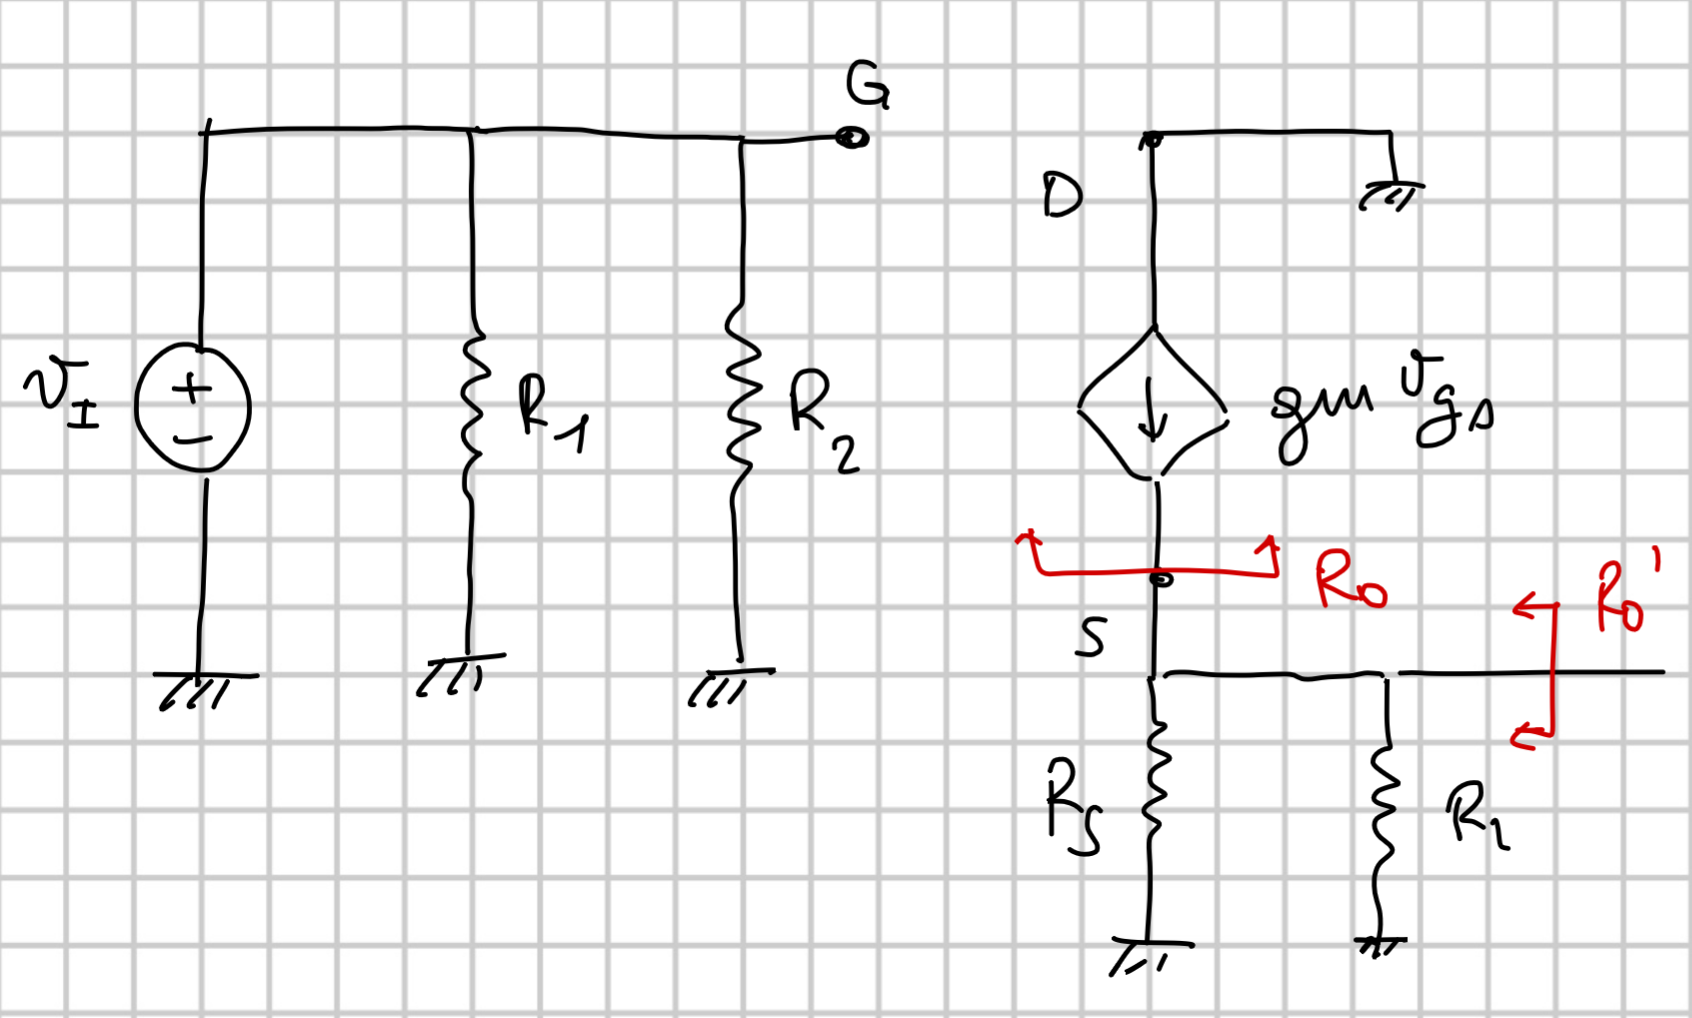
\includegraphics[scale=0.15]{../figures/mosfet_drain_imane.png}
\end{center}

Calcoliamo anche qui i parametri caratteristici:
\begin{itemize}
\item \textbf{\textsf{Guadagno di tensione}} $A_v$ \\
Per calcolare il guadagno di tensione, come sopra, prendiamo il rapporto fra tensione di uscita e tensione di ingresso. La prima fra queste si calcolerà come:
$$
v_o = g_m v_{gs} R_S 
$$
dove consideriamo la $v_{gs}$:
$$
\begin{cases}
v_g = v_i \\
v_s = v_o 
\end{cases}, \quad
v_{gs} = v_g - v_o
$$
che ci dà:
$$
v_o = g_m (v_g - v_o) R_S \implies v_o = \frac{g_m v_i R_S}{1 + g_m R_S} 
$$
e quindi il rapporto complessivo è:
$$
A_v = \frac{v_o}{v_i} \Big|_{R_L \rightarrow \infty} = \frac{g_m R_s}{1 + g_m R_S}
$$

Anche qui abbiamo ottenuto una configurazione simile all'equivalente nel BJT (a collettore comune), cioè abbiamo una configurazione \textit{source follower} dove, se $g_m R_s >> 1$, $A_v \approx 1$ e si replica il segnale di ingresso all'uscita così com'è, ma a bassa impedenza (il cosiddetto elemento di \textit{buffer}).

\item \textbf{\textsf{Guadagno di corrente}} $A_i$ \\
Abbiamo detto che lo stage di ingresso non cambia, per cui non cambiano né impedenza all'ingresso ($\rightarrow \infty$) ne corrente allo stadio di ingresso ($0$) e quindi:
$$
A_i \rightarrow = \infty
$$

\item \textbf{\textsf{Impedenza in uscita}} $R_o$ \\
La resistenza in uscita si calcola imponendo la tensione di prova $v_P$ all'uscita (al source del MOSFET), e spegnendo il segnale in ingresso, per cui:
$$
\begin{cases}
v_g = 0 \\
v_s = v_P
\end{cases}, \quad
v_{gs} = v_g - v_s = - v_P 
$$
e la corrente:
$$
i_p - g_m v_{gs} = g_m v_P
$$
da cui si ha quindi:
$$
R_o = \frac{1}{g_m}
$$
e cioè la resistenza in uscita è l'inverso della conduttanza differenziale.

La resistenza a valle di $R_L$ e $R_S$ chiaramente sarà data dal parallelo:
$$
\frac{1}{g_m} || R_S || R_L
$$

Notando poi che $g_m$ è solitamente piccola, si ha che la resistenza complessiva in uscita della configurazione a drain comune è piuttosto piccola.

\item \textbf{\textsf{Impedenza in ingresso}} $R_i$ \\
Visto che lo stage di ingresso non cambia, questa rimane:
$$
R_i \rightarrow \infty
$$
\end{itemize}

\par\smallskip

Come per i transistori BJT, il MOSFET ha una configurazione a gate comune (per il BJT era a base comune), che però non vediamo (la derivazione sarà comunque analoga a queste).

\subsection{Amplificatori multistadio}
Per concludere l'argomento degli amplificatori, vediamo che solitamente nelle applicazioni reali si combinano più reti amplificatrici in cascata (che denominiamo \textit{stadi} o \textit{stage} di amplificazione). Ogni rete avrà il compito di compiere un passaggio dell'amplificazione del segnale, indipendentemente dalle altre.

Poniamo di avere ad esempio un amplificatore a 2 stadi:
\begin{enumerate}
	\item Stadio 1, con le proprie $R_{i1}$, $R_{o1}$ e $A_{v1}$;
	\item Stadio 2, con le proprie $R_{i2}$, $R_{o2}$ e $A_{v2}$
\end{enumerate}
Il circuito con gli stadi in cascata sarà ad esempio il seguente:

\begin{center}
\begin{tikzpicture}[transform shape]
	% Paths, nodes and wires:
	\node[shape=rectangle, draw, line width=1pt, minimum width=1.965cm, minimum height=2.465cm] at (3, 5){} node[anchor=center, align=center, text width=1.577cm, inner sep=6pt] at (3, 5){\footnotesize Amp. 1\\$R_{i1}$ $R_{o1}$ $A_{v1}$};
	\draw (0, 4) -- (2, 4);
	\draw (4, 6) -- (6, 6);
	\draw (4, 4) -- (6, 4);
	\draw (8, 6) -- (10, 6);
	\draw (8, 4) -- (10, 4);
	\node[shape=rectangle, draw, line width=1pt, minimum width=1.965cm, minimum height=2.465cm] at (7, 5){} node[anchor=center, align=center, text width=1.577cm, inner sep=6pt] at (7, 5){\footnotesize Amp. 2\\$R_{i2}$ $R_{o2}$ $A_{v2}$};
	\draw (10, 6) to[american resistor, l_={$R_L$}, v^=$V_u$, voltage=american] (10, 4);
	\draw (0, 6) to[american resistor, l={$R_s$}] (2, 6);
	\draw (0, 4) to[european voltage source, l={$V_i$}] (0, 6);
\end{tikzpicture}
\end{center}

La domanda che ci poniamo è chiaramente come si combinano i parametri di amplificazione, e in particolare il guadagno di tensione $A_v$ complessivo, che è ciò che ci interessa da un amplificatore.

Notiamo che di base vale che:
$$
A_v = \frac{V_o}{V_i} = A_{v1} A_{v2}
$$
cioè generalmente il guadagno non è dato dal guadagno sulla seconda rete della prima rete.

Dobbiamo quindi usare la rappresentazione a parametri equivalenti dei 2 stadi per avere una risposta più accurata.

\begin{center}
\begin{tikzpicture}[transform shape]
	% Paths, nodes and wires:
	\draw (-0, 4) -- (2, 4);
	\draw (6, 6) -- (8, 6);
	\draw (6, 4) -- (8, 4);
	\draw (12, 6) -| (13, 6);
	\draw (12, 4) -- (13, 4);
	\draw (13, 6) to[american resistor, l_={$R_L$}, v^=$V_u$, voltage=american] (13, 4);
	\draw (-0, 6) to[american resistor, l={$R_s$}] (2, 6);
	\draw (-0, 4) to[european voltage source, l={$V_i$}] (-0, 6);
	\draw (2.5, 6) to[american resistor, l={$R_{i1}$}] (2.5, 4);
	\draw (4, 6) to[american resistor, l={$R_{o1}$}] (6, 6);
	\draw (4, 6) to[american controlled voltage source, l={$A_{v1}v_1$}] (4, 4);
	\draw (2, 6) -- (2.5, 6);
	\draw (2, 4) -- (2.5, 4);
	\draw (4, 4) -- (6, 4);
	\draw (8.5, 6) to[american resistor, l={$R_{i2}$}] (8.5, 4);
	\draw (10, 6) to[american resistor, l={$R_{o2}$}] (12, 6);
	\draw (10, 6) to[american controlled voltage source, l={$A_{v2}v_2$}] (10, 4);
	\draw (8, 6) -- (8.5, 6);
	\draw (8, 4) -- (8.5, 4);
	\draw (10, 4) -- (12, 4);
	\draw (2, 6) to[open, v=$v_1$, voltage=american] (2, 4);
	\draw (7, 6) to[open, v=$v_1$, voltage=american] (7, 4);
	\node[shape=rectangle, draw, line width=0.5pt, dash pattern={on 2pt off 2pt}, minimum width=3.982cm, minimum height=3.982cm] at (4, 5){};
	\node[shape=rectangle, draw, line width=0.5pt, dash pattern={on 2pt off 2pt}, minimum width=3.982cm, minimum height=3.982cm] at (10, 5){};
	\node[shape=rectangle, minimum width=3.965cm, minimum height=0.465cm] at (4, 7.25){} node[anchor=center, align=center, text width=3.577cm, inner sep=6pt] at (4, 7.25){Amp. 1};
	\node[shape=rectangle, minimum width=3.965cm, minimum height=0.465cm] at (10, 7.25){} node[anchor=center, align=center, text width=3.577cm, inner sep=6pt] at (10, 7.25){Amp. 1};
\end{tikzpicture}
\end{center}

Calcoliamo quindi il guadagno in tensione complessivo come il rapporto fra la tensione in uscita a valle di entrambi gli stadi, e la tensione fornita in ingresso:
$$
A_v = \frac{V_o}{V_i} \Big|_{R_L \rightarrow \infty}
$$
dove varrà:
$$
V_o = A_{V2} V_{i2}, \quad V_{i2} = (A_{v1} V_{i1}) \frac{R_{i2}}{R_{i2} + R_{o1}}
$$
Notando che $V_{i1} = V_i$ si ricava quindi:
$$
A_v = \frac{V_o}{V_i} \Big|_{R_L \rightarrow \infty} = (A_{v1} A_{v2}) {R_{i2} + R_{o1}}
$$
cioè si prende il risultato che immaginavamo ($A_{v1} A_{v2}$), ma moltiplicato per il termine (${R_{i2} + R_{o1}}$). 

Questo termine è conseguenza dell'\textit{interazione} fra i 2 stadi. Si dice in particolare che lo stadio 1 \textit{carica} lo stadio 2. Questo è immediata conseguenza del fatto che nel calcolo dei parametri abbiamo assunto impedenza in uscita infinita, mentre nel caso reale l'impedenza a valle di uno stadio è chiaramente quella in ingresso dello stadio successivo.

Perché le formule obbediscano alla formula che vogliamo, quindi (cioè $A_{v1} A_{v2}$) dovremmo imporre una cosa del tipo:
$$
R_{i2} \rightarrow \infty \ \text{oppure} \ R_{o1} \rightarrow 0
$$
cioè in generale vogliamo stadi con alta impedenza in ingresso e bassa impedenza in uscita.
\begin{itemize}
	\item L'alta impedenza in ingresso presuppone che uno stadio non carichi il precedente, cioè "\textit{campioni}" il voltaggio senza concedere cadute di tensione date dal passaggio di corrente;
	\item La bassa impedenza in uscita serve invece per poter pilotare in maniera efficiente gli stadi a monte.
\end{itemize}

Questa linea di pensiero non è esclusiva agli amplificatori ma riguarda ogni circuito di elaborazione di segnale che andrà messo in cascata con altri circuiti a porte simili.


\end{document}
